%==========================================================
%
% Formalizing Theorems with PVS
%
% Summer UnB
%
% Jan 17 - 21, 2022
%
%==========================================================
%==========================================================
\documentclass[10pt]{beamer}
\usepackage[utf8]{inputenc}
%\usepackage[brazil]{babel}
\usepackage{multicol}
\usepackage{amssymb}
\usepackage{amsmath}
\usepackage{graphicx}
\usepackage{xcolor}
\usepackage{mathtools}
\usepackage{mathrsfs}
\usepackage{fancyvrb}
\usepackage[all,2cell]{xy}
\usepackage{proof}  
\usepackage{mathpartir}
\usepackage{tikz}
\usetikzlibrary{arrows,snakes,backgrounds}
\usepackage{pdfsync}
\synctex=1

%==========================================================
%==========================================================
\usecolortheme[cmyk={0.8,0.3,0,0.6}]{structure}
    \usetheme[secheader]{Boadilla}         
    \setbeamertemplate{footline}
        {
      \leavevmode%
      \hbox{%
\begin{beamercolorbox}[wd=.333333\paperwidth,ht=2.25ex,dp=1ex,center]{author in head/foot}%
        \usebeamerfont{author in head/foot}\insertshortauthor~~%(\insertshortinstitute)
      \end{beamercolorbox}%
\begin{beamercolorbox}[wd=.333333\paperwidth,ht=2.25ex,dp=1ex,center]{title in head/foot}%
        \usebeamerfont{title in head/foot}\insertshorttitle
      \end{beamercolorbox}%
\begin{beamercolorbox}[wd=.333333\paperwidth,ht=2.25ex,dp=1ex,right]{date in head/foot}%
        \usebeamerfont{date in head/foot}\insertshortdate{}\hspace*{2em}
      \end{beamercolorbox}}%
      \vskip0pt%
    }
\usefonttheme[onlymath]{serif}
\setbeamertemplate{theorems}[numbered]    
%==========================================================
%==========================================================
%==========================================================
\newtheorem{teorema}{Teorema}[section]
\newtheorem{corolario}[teorema]{Corol\'{a}rio}
\newtheorem{lema}[teorema]{Lema}
\newtheorem{proposicao}[teorema]{Proposi\c{c}\~{a}o}
\newcommand{\demonstracao}{\noindent {\color{red}{Demonstra\c{c}\~{a}o:}} }
\newtheorem{definicao}[teorema]{Defini\c{c}\~{a}o}
%==========================================================
\newtheorem{exemplo}{Exemplo}[section]
\newtheorem{exemplos}[exemplo]{Exemplos}
\newtheorem{nota}{Nota}[section]
\newtheorem{observacao}[nota]{Observa\c{c}\~{a}o}
\newtheorem{notacao}[nota]{Nota\c{c}\~{a}o}
%==========================================================
%==========================================================
%==========================================================
\newcommand{\bck}[0]{$\backslash$}
\newcommand{\ttblue}[1]{{\color{blue!80!black}\tt#1}}
\newcommand{\ttbe}[1]{{\color{blue!80!black}\tt\emph{#1}}}
\definecolor{aquamarine}{rgb}{0.5, 1.0, 0.83}
\definecolor{darkorange}{rgb}{1.0, 0.55, 0.0}
\newcommand{\op}[1]{_{\scriptscriptstyle{#1}}}
\newcommand{\ttdo}[1]{{\color{darkorange}\tt#1}}
\newcommand{\ttaq}[1]{{\color{aquamarine}\tt#1}}
\newcommand{\boxdarkgray}[1]{\fbox{\color{darkgray}{#1}}}
\linespread{1.3}
%==========================================================
% new commands ISR2018
%==========================================================
\newcommand{\deriv}{\bigtriangledown}
\newcommand{\cut}{\mm{(Cut)}}
\newcommand{\toesm}{\mm{(\to_e)}}
\newcommand{\toism}[1]{\mm{(\to_i){#1}}}
\newcommand{\toe}{\mm{(\to_e)}}
\newcommand{\toisa}{\mm{(\to_i)}}
\newcommand{\toi}[1]{\mm{(\to_i)\;{#1}}}
\newcommand{\landi}{\mm{(\land_i)}}
\newcommand{\lande}{\mm{(\land_e)}}
\newcommand{\landef}{\mm{(\land_{e_1})}}
\newcommand{\landes}{\mm{(\land_{e_2})}}
\newcommand{\lorif}{\mm{(\lor_{i_1})}}
\newcommand{\loris}{\mm{(\lor_{i_2})}}
\newcommand{\lori}{\mm{(\lor_i)}}
\newcommand{\lore}[2]{\mm{(\lor_e)\;{#1},{#2}}}
\newcommand{\loresa}{\mm{(\lor_e)}}
\newcommand{\loresm}[2]{\mm{(\lor_e)\;{#1},{#2}}}
\newcommand{\nege}{\mm{(\neg_e)}}
\newcommand{\negi}[1]{\mm{(\neg_i)\;{#1}}}
\newcommand{\negisa}{\mm{(\neg_i)}}
\newcommand{\nne}{\mm{(\neg\neg_e)}}
\newcommand{\nni}{\mm{(\neg\neg_i)}}
\newcommand{\nnesm}{\mm{(\neg\neg_e)}}
\newcommand{\nnism}{\mm{(\neg\neg_i)}}
\newcommand{\lem}{\rm{LEM}}
\newcommand{\pair}[2]{\mm{\langle #1, #2 \rangle}}
\newcommand{\pbc}[1]{\mm{({\rm PBC})\;{#1}}}
\newcommand{\pbcsm}[1]{(\rm{PBC}),#1}
\newcommand{\pbcsa}{(\rm{PBC})}
\newcommand{\lemcp}{(\rm{LEM})}
\newcommand{\mt}{\rm{MT}}
\newcommand{\bote}{\mm{(\bot_e)}}
\newcommand{\botesm}{\mm{(\bot_e)}}
\newcommand{\nat}{\mm{\mathbb{N}}}
\newcommand{\add}{\mm{\tt +}}
\newcommand{\lb}{\mm{\lambda}}
\newcommand{\alle}{\mm{(\forall_e)}}
\newcommand{\alli}{\mm{(\forall_i)}}
\newcommand{\exie}[1]{\mm{(\exists_e)\;{#1}}}
\newcommand{\exii}{\mm{(\exists_i)}}
\newcommand{\true}{\mm{ T}}
\newcommand{\false}{\mm{ F}}
\newcommand{\m}{{\tt m}}
\newcommand{\z}{{\tt z}}
\newcommand{\pseq}{\mbox{{\tt |---}\;}} 

\newcommand{\var}{{\sc (Var)}}
\newcommand{\app}{{\sc (App)}}
\newcommand{\absA}{{\sc (Abs)}}
\newcommand{\imp}{\to}
\newcommand{\axiom}{{\sc (axiom)}} 
\newcommand{\axiomvar}{{\sc (axiom\ var)}} 
\newcommand{\axiomtop}{{\sc (axiom\ $\top$)}} 
\newcommand{\axiombot}{{\sc (axiom\ $\bot$)}} 
\newcommand{\negation}{{\sc (negation)}} 
\newcommand{\conjunction}{{\sc (conjunction)}} 
\newcommand{\disjunction}{{\sc (disjunction)}} 
\newcommand{\implication}{{\sc (implication)}} 
\newcommand{\prop}{\rm{Prop}}
\newcommand{\tvarset}{\mathbb{V}}
\newcommand{\funset}{\mathbb{F}}
\newcommand{\predset}{\mathbb{P}}
\newcommand{\dom}{\mm{\tt D}}
\newcommand{\fv}[1]{{\tt fv}(#1)}
\newcommand{\bv}[1]{{\tt bv}(#1)}
\newcommand{\set}[1]{ \{ #1 \}}
\renewcommand{\min}[1]{ {min \{ #1 \}}}
\newcommand{\vars}[1]{\mm{{\tt var}(#1)}}
\newcommand{\subs}[2]{ \{ #1/#2 \}}
\newcommand{\fosubs}[2]{ [#1/#2]}




% Begin Commands Talk Verao 2007
\newcommand{\myboxvariable}[3]{\vspace{-3mm}$$\vbox{\hrule\hbox{\vrule\hskip#1\vbox{\vskip#1{}\hsize=#2\hsize\noindent#3\vskip#1}\hskip#1\vrule}\hrule}\vspace{-3.7mm}$$}
\newcommand\mdc{\mbox{\it gcd}}
\newcommand\LDB{\Lambda_{dB}}
\newcommand{\fd}{\to}
\newcommand{\abst}[3]{\lambda {#1}{:}{#2}.{#3}}
\newcommand\FV{{\mathcal FV}}
\newcommand\sub[3]{{#1}\{{#2}/{#3}\}}
\newcommand{\SEL}[1]{(\lambda #1)}
\newcommand{\SEA}[2]{(#1\;#2)}
\newcommand{\SEDB}[1]{{\tt \underline{#1}}}
\newcommand{\SEVr}[1]{#1}
\newcommand{\SESb}[2]{#1[#2]}
\newcommand{\SES}[3]{(#2\sigma^{#1}#3)}
\newcommand{\SEP}[3]{\varphi^{#1}_{#2}(#3)}
\newcommand{\SEDummy}{\diammond}
\newcommand{\SESp}[4]{[\![#1,#2,#3,#4]\!]}
\newcommand{\SEId}{id}
\newcommand{\SEUp}{\uparrow}
\newcommand{\SEPt}[2]{(#1\cdot #2)}
\newcommand{\SECp}[2]{(#1\circ#2)}
\newcommand{\SECon}[2]{#1::#2}
\newcommand{\SECk}[4]{\{\!\{#1,#2,#3,#4\}\!\}}
\newcommand{\SENil}{nil}
\newcommand{\SEPaar}[2]{(#1,#2)}
\newcommand{\SEAr}[1]{@#1}
\newcommand{\SELG}[4]{\langle\!\langle#1,#2,#3,#4\rangle\!
angle}


\newcommand{\rTo}{\longrightarrow}

\newcommand{\abs}[2]{\lambda_{#1}.{#2}}
\newcommand{\absG}[2]{\mbox{\color{\FigGcol}$\lambda_{#1}.{#2}$}}
\newcommand{\absR}[2]{\mbox{\color{\FigRcol}$\lambda_{#1}.{#2}$}}
\newcommand{\absB}[2]{\mbox{\color{\FigBcol}$\lambda_{#1}.{#2}$}}
\newcommand{\tyabs}[2]{\lambda_{#1}.{#2}}
\newcommand{\absb}[1]{\lambda.{#1}}
\newcommand{\absbG}[1]{\mbox{\color{\FigGcol}$\lambda.{#1}$}}
\newcommand{\absbR}[1]{\mbox{\color{\FigRcol}$\lambda.{#1}$}}
\newcommand{\absbB}[1]{\mbox{\color{\FigBcol}$\lambda.{#1}$}}
\newcommand{\absdb}[1]{\lambda {#1}}
\newcommand{\apl}[2]{({#1}\;\;{#2})}
\newcommand{\myigls}{=_{\lambda s_e}^?}
\newcommand{\igls}{=_{\lambda\sigma}^?}
\newcommand{\tvar}{{\it {\cal T}var}}
\newcommand\Sub[2]{{#1}[{#2}]}
\newcommand\Id{id}
\newcommand\Comp[2]{{#1} \circ {#2}}
\newcommand\Sh{\uparrow}
\newcommand{\substit}{{\it Subst}}
\newcommand{\vvar}{{\it var}}
\newcommand{\fvar}{{\it {\cal F}var}}
\newcommand{\beigls}{=_{\beta\eta}^?}
\newcommand \si {\,\sigma^i}
\newcommand \fik {\varphi^i_k}
\newcommand{\AND}{\ {\wedge}\ }
\newcommand{\OR}{\ {\vee}\ }
\newcommand{\IMPLIES}{\ {\Rightarrow}\ }
\newcommand{\NOT}{\neg}

%==========================================================

\title
[Mechanizing Mathematics]
{\vspace{-5mm}
%\includegraphics[scale=.35]{Marca_UFG.png}
\\%[8mm]
%{\scriptsize\bf  Universidad Nacional de Colombia - Sede Manizales}\\
{\bf\Large Mechanizing Mathematics}\\
{\large Mathematical Deduction} \vspace{-.1cm}}


\author[M. Ayala-Rinc\'on (UnB) \& T. A. de Lima (UFG)]
{Universidad Nacional de Colombia - Sede Manizales \\
Facultad de Ciencias Exactas y Naturales\\[6mm]
\textbf{Thaynara Arielly de Lima
  (IME)}   
\includegraphics[scale=.18]{ufg.png}\\
\textbf{Mauricio Ayala-Rinc\'on (CIC-MAT)} 
\includegraphics[scale=.03]{unb.jpg}
\vspace{-.8cm}}

\date[Universidad Nacional de Colombia - Sede Manizales]{{\scriptsize\it Funded by the Brazilian agencies CNPq, grants Universal 409003/21-2; \\ FAPDF, grant DE 00193-00001175/2021-11 and \\ FAPEG, grant 202310267000223.}
\\ May 29 - June 02 ,
  2023}  



\pgfdeclareimage[height=2.0cm]{deBruijn}{figs/deBruijn}
\pgfdeclareimage[height=2.0cm]{Landau}{figs/EdmundLandau}
\pgfdeclareimage[height=3.5cm]{35Years}{figs/35YearsAutomath}
\pgfdeclareimage[height=1cm]{35YearsA}{figs/35YearsAutomath}
\pgfdeclareimage[height=3.5cm]{SelectedAutomath}{figs/SelectedAutomath}
\pgfdeclareimage[height=2cm]{CurryHoward}{figs/CurryHoward}
\pgfdeclareimage[height=1cm]{AutomathHeader}{figs/AutomathHeader}
\pgfdeclareimage[height=2.5cm]{KnuthSelectedPapersonAlgorithms}{figs/KnuthSelectedPapersonAlgorithms}
\pgfdeclareimage[height=2.5cm]{KnuthdeBruijn}{figs/KnuthdeBruijn}
\pgfdeclareimage[height=2.0cm]{VladimirVoevodsky}{figs/VladimirVoevodsky} 
\pgfdeclareimage[height=0.8cm]{FieldMedal}{figs/FieldMedal} 
\pgfdeclareimage[height=2.5cm]{GrundlageAnalysiscapa}{figs/GrundlageAnalysiscapa}
\pgfdeclareimage[height=3.5cm]{HottBook}{figs/HottBook} 
\pgfdeclareimage[height=3.5cm]{ITPcapa}{figs/ITPcapa} 
\pgfdeclareimage[height=3.5cm]{MSCScapa}{figs/MSCScapa} 
\pgfdeclareimage[height=3.5cm]{TCScapa}{figs/TCScapa} 
\pgfdeclareimage[height=3.5cm]{JARcapa}{figs/JARcapa} 
\pgfdeclareimage[height=3.5cm]{LJIGPLcapa}{figs/LJIGPLcapa} 
\pgfdeclareimage[height=3.5cm]{SCPcapa}{figs/SCPcapa}
\pgfdeclareimage[height=3.5cm]{SciComProgCover}{figs/SciComProgCover}
\pgfdeclareimage[height=3.5cm]{WoLLICcapa}{figs/WoLLICcapa} 
\pgfdeclareimage[height=3.5cm]{ENTCScapa}{figs/ENTCScapa} 
\pgfdeclareimage[height=3.5cm]{LOPSTRcapa}{figs/LOPSTRcapa} 
\pgfdeclareimage[height=3.5cm]{LMCScapa}{figs/LMCScapa}
\pgfdeclareimage[height=3.1cm]{LogforCScapa}{figs/LogforCScapa}
\pgfdeclareimage[height=3.1cm]{Logiccapa}{figs/Logiccapa} 
\pgfdeclareimage[height=3.1cm]{ProofTheorycapa}{figs/ProofTheorycapa} 
\pgfdeclareimage[height=3.1cm]{TypeTheorycapa}{figs/TypeTheorycapa} 
\pgfdeclareimage[height=3.1cm]{Rewritingcapa}{figs/Rewritingcapa} 

\pgfdeclareimage[height=0.5cm]{LIPIcscapita}{figs/LIPIcsCapa}
\pgfdeclareimage[height=0.5cm]{ITPcapita}{figs/ITPcapa}
\pgfdeclareimage[height=0.5cm]{SciComProgCapita}{figs/SciComProgCover}
\pgfdeclareimage[height=0.5cm]{MSCScapita}{figs/MSCScapa} 
\pgfdeclareimage[height=0.5cm]{TCScapita}{figs/TCScapa} 
\pgfdeclareimage[height=0.5cm]{JARcapita}{figs/JARcapa} 
\pgfdeclareimage[height=0.5cm]{LJIGPLcapita}{figs/LJIGPLcapa} 
\pgfdeclareimage[height=0.5cm]{SCPcapita}{figs/SCPcapa} 
\pgfdeclareimage[height=0.5cm]{WoLLICcapita}{figs/WoLLICcapa} 
\pgfdeclareimage[height=0.5cm]{ENTCScapita}{figs/ENTCScapa} 
\pgfdeclareimage[height=0.5cm]{LOPSTRcapita}{figs/LOPSTRcapa} 
\pgfdeclareimage[height=0.5cm]{LMCScapita}{figs/LMCScapa} 

%==========================================================
%==========================================================
\begin{document}
%==========================================================
%==========================================================
\begin{frame}
\maketitle
\end{frame}
%==========================================================
%==========================================================
\begin{frame}
\frametitle{Talk's Plan}
%----------------------------------------
\begin{columns}
\begin{column}{10cm}
%----------------------------------------
\tableofcontents
%----------------------------------------
\end{column}
\end{columns}
%----------------------------------------
\end{frame}




%==========================================================
%==========================================================

%==========================================================
%==========================================================

%%% ==============
%%% ==============
% Propaganda
%%% ==============
%%% ==============




%==========================================================
%==========================================================

\section{Formalizing Mathematics}

\begin{frame}
\frametitle{Formalizing Mathematics}
%----------------------------------------
Since the early development of computers, implementing mathematical
deduction was a very important challenge:

\begin{columns}
\begin{column}{0.5\textwidth}  Nicolaas Govert de Bruijn
  (1918-2012). Dutch mathematician leader of the  {\color{blue}
    Automath} project.\end{column}
\begin{column}{0.1\textwidth}  \pgfuseimage{deBruijn} \end{column}\end{columns}

\vspace{1cm}


{\color{blue} Automath} started in 1967:  

\vspace{3mm}

\begin{columns}
\begin{column}{0.1\textwidth} \pgfuseimage{Landau}  \end{column} \begin{column}{0.5\textwidth} Mechanical verification of the famous Edmund
Landau's  (1877-1938) book \emph{Grundlagen der Analysis}, Leipzig
1930.\end{column}
\begin{column}{0.1\textwidth} \pgfuseimage{GrundlageAnalysiscapa}  \end{column} 
\end{columns}

 


\end{frame}


\begin{frame}\frametitle{Formalizing Mathematics}



\begin{columns}
\begin{column}{0.45\textwidth}
  \pgfuseimage{AutomathHeader} \end{column}
\begin{column}{0.49\textwidth} \url{https://www.win.tue.nl/automath/}
\end{column}
\end{columns}

\vspace{1cm}

\begin{columns}
\begin{column}{0.4\textwidth} {\color{blue} Automath} is considered predecessor of modern
  proof assistants as: {\color{blue} Coq}, {\color{blue} Nurpl},
  {\color{blue} Isabelle}, {\color{blue} PVS} ...
\end{column}
\begin{column}{0.2\textwidth} 
\pgfuseimage{35Years}   
\end{column}
\begin{column}{0.2\textwidth} 
  \pgfuseimage{SelectedAutomath} 
\end{column}
\end{columns}


\end{frame}



\begin{frame}
\frametitle{Formalizing Mathematics}

\begin{columns}
\begin{column}{0.7\textwidth}  In  {\color{blue} Automath} N.G. de Bruijn developed the first
  formalization of  $\lambda$-calculus with {\color{cyan} intuitionistic types} and
 {\color{cyan} explicit substitutions}. \end{column}
\begin{column}{0.1\textwidth}  \pgfuseimage{deBruijn} \end{column}\end{columns}


\vspace{.5cm}



\begin{columns}
\begin{column}{0.2\textwidth} \pgfuseimage{35Years} \end{column}
\begin{column}{0.7\textwidth} 
\emph{\footnotesize\color{blue}
N.G. de Bruijn was a well established mathematician before deciding in
1967 at the age of 49 to work on a new direction related to Automating
Mathematics. In the 1960s he became fascinated by the new computer
technology and decided to start the new Automath project where he
could check, with the help of the computer, the correctness of books
of mathematics. Through his work on Automath, de Bruijn started a
revolution in using the computer for verification, and since, we have
seen more and more proof-checking and theorem-proving systems. }
\end{column}\end{columns}


\end{frame}

\begin{frame}
\frametitle{Formalizing Mathematics}

N.G. De Bruijn's influence in computing is not restricted to
{\color{blue} Automath}.

\vspace{5mm}

\begin{columns}
\begin{column}{0.2\textwidth} \pgfuseimage{KnuthSelectedPapersonAlgorithms}
\end{column}
\begin{column}{0.7\textwidth}
\footnotesize{ Donald Knuth dedicates his book to his mentor, N. G. de Bruijn.}
\end{column}
\end{columns}

\vspace{5mm}

\begin{columns}
\begin{column}{0.2\textwidth} \pgfuseimage{KnuthdeBruijn}
          \end{column}
  \begin{column}{0.7\textwidth}         {\scriptsize\em \color{blue}
... I'm dedicating this book to N.G. ``Dick'' de Bruijn
because his influence can be felt on every page.
Ever since the 1960s he has been my chief mentor, the main
person who would answer my questions when I was stuck on a
problem that I had not been taught how to solve. 
I originally wrote Chapter 26 for his $(3\cdot 4\cdot 5)$th birthday;
now he is $3^4$ years young as I gratefully present him with
this book. 
\hfill {\color{black}Donald E. Knuth}
     }
\end{column}
\end{columns}



\end{frame}



\begin{frame}\frametitle{Formalizing Mathematics}



\begin{columns}
\begin{column}{0.2\textwidth}\pgfuseimage{VladimirVoevodsky} 
\end{column}
\begin{column}{0.6\textwidth} Vladimir Voevodsky (1966-2017) (\pgfuseimage{FieldMedal} 2002) popularised the {\color{blue}
    Univalent Foundations} that use classical predicate logic as the
  underlying deductive sytem, categorical approaches, and intuitionistic types,
  indeed the so called
\end{column}
\end{columns}

\vspace{5mm}

\begin{columns}
\begin{column}{0.5\textwidth} \url{https://homotopytypetheory.org}
\end{column}
\begin{column}{0.4\textwidth}\pgfuseimage{HottBook}   \end{column}
\end{columns}

\end{frame}


\begin{frame}\frametitle{Formalizing Mathematics today}


  \begin{columns}
\begin{column}{0.3\textwidth}\href{http://dx.doi.org/10.1090/noti1688}{\color{blue}
  \scriptsize{Jeremy Avigad  {\it ``The Mechanization of
      Mathematics''}} - Notices of the ACM 2018}
\end{column}

\begin{column}{0.6\textwidth}
  \small{Avigad given  examples are {\it ``signs that such mechanical tools will allow
a fundamental expansion of our capacities for discovering, verifying,
and communicating mathematical knowledge.''}

\vspace{5mm}

{\it ``The history of mathematics is a history of doing whatever
it takes to extend our cognitive reach, and designing
concepts and methods that augment our capacities to
understand. The computer is nothing more than a tool
in that respect, but it is one that fundamentally expands
the range of structures we can discover and the kinds of
truths we can reliably come to know.''}
}
\end{column}
\end{columns}

\end{frame}  

\begin{frame}\frametitle{Formalizing Mathematics today}


  \begin{columns}
\begin{column}{0.45\textwidth}
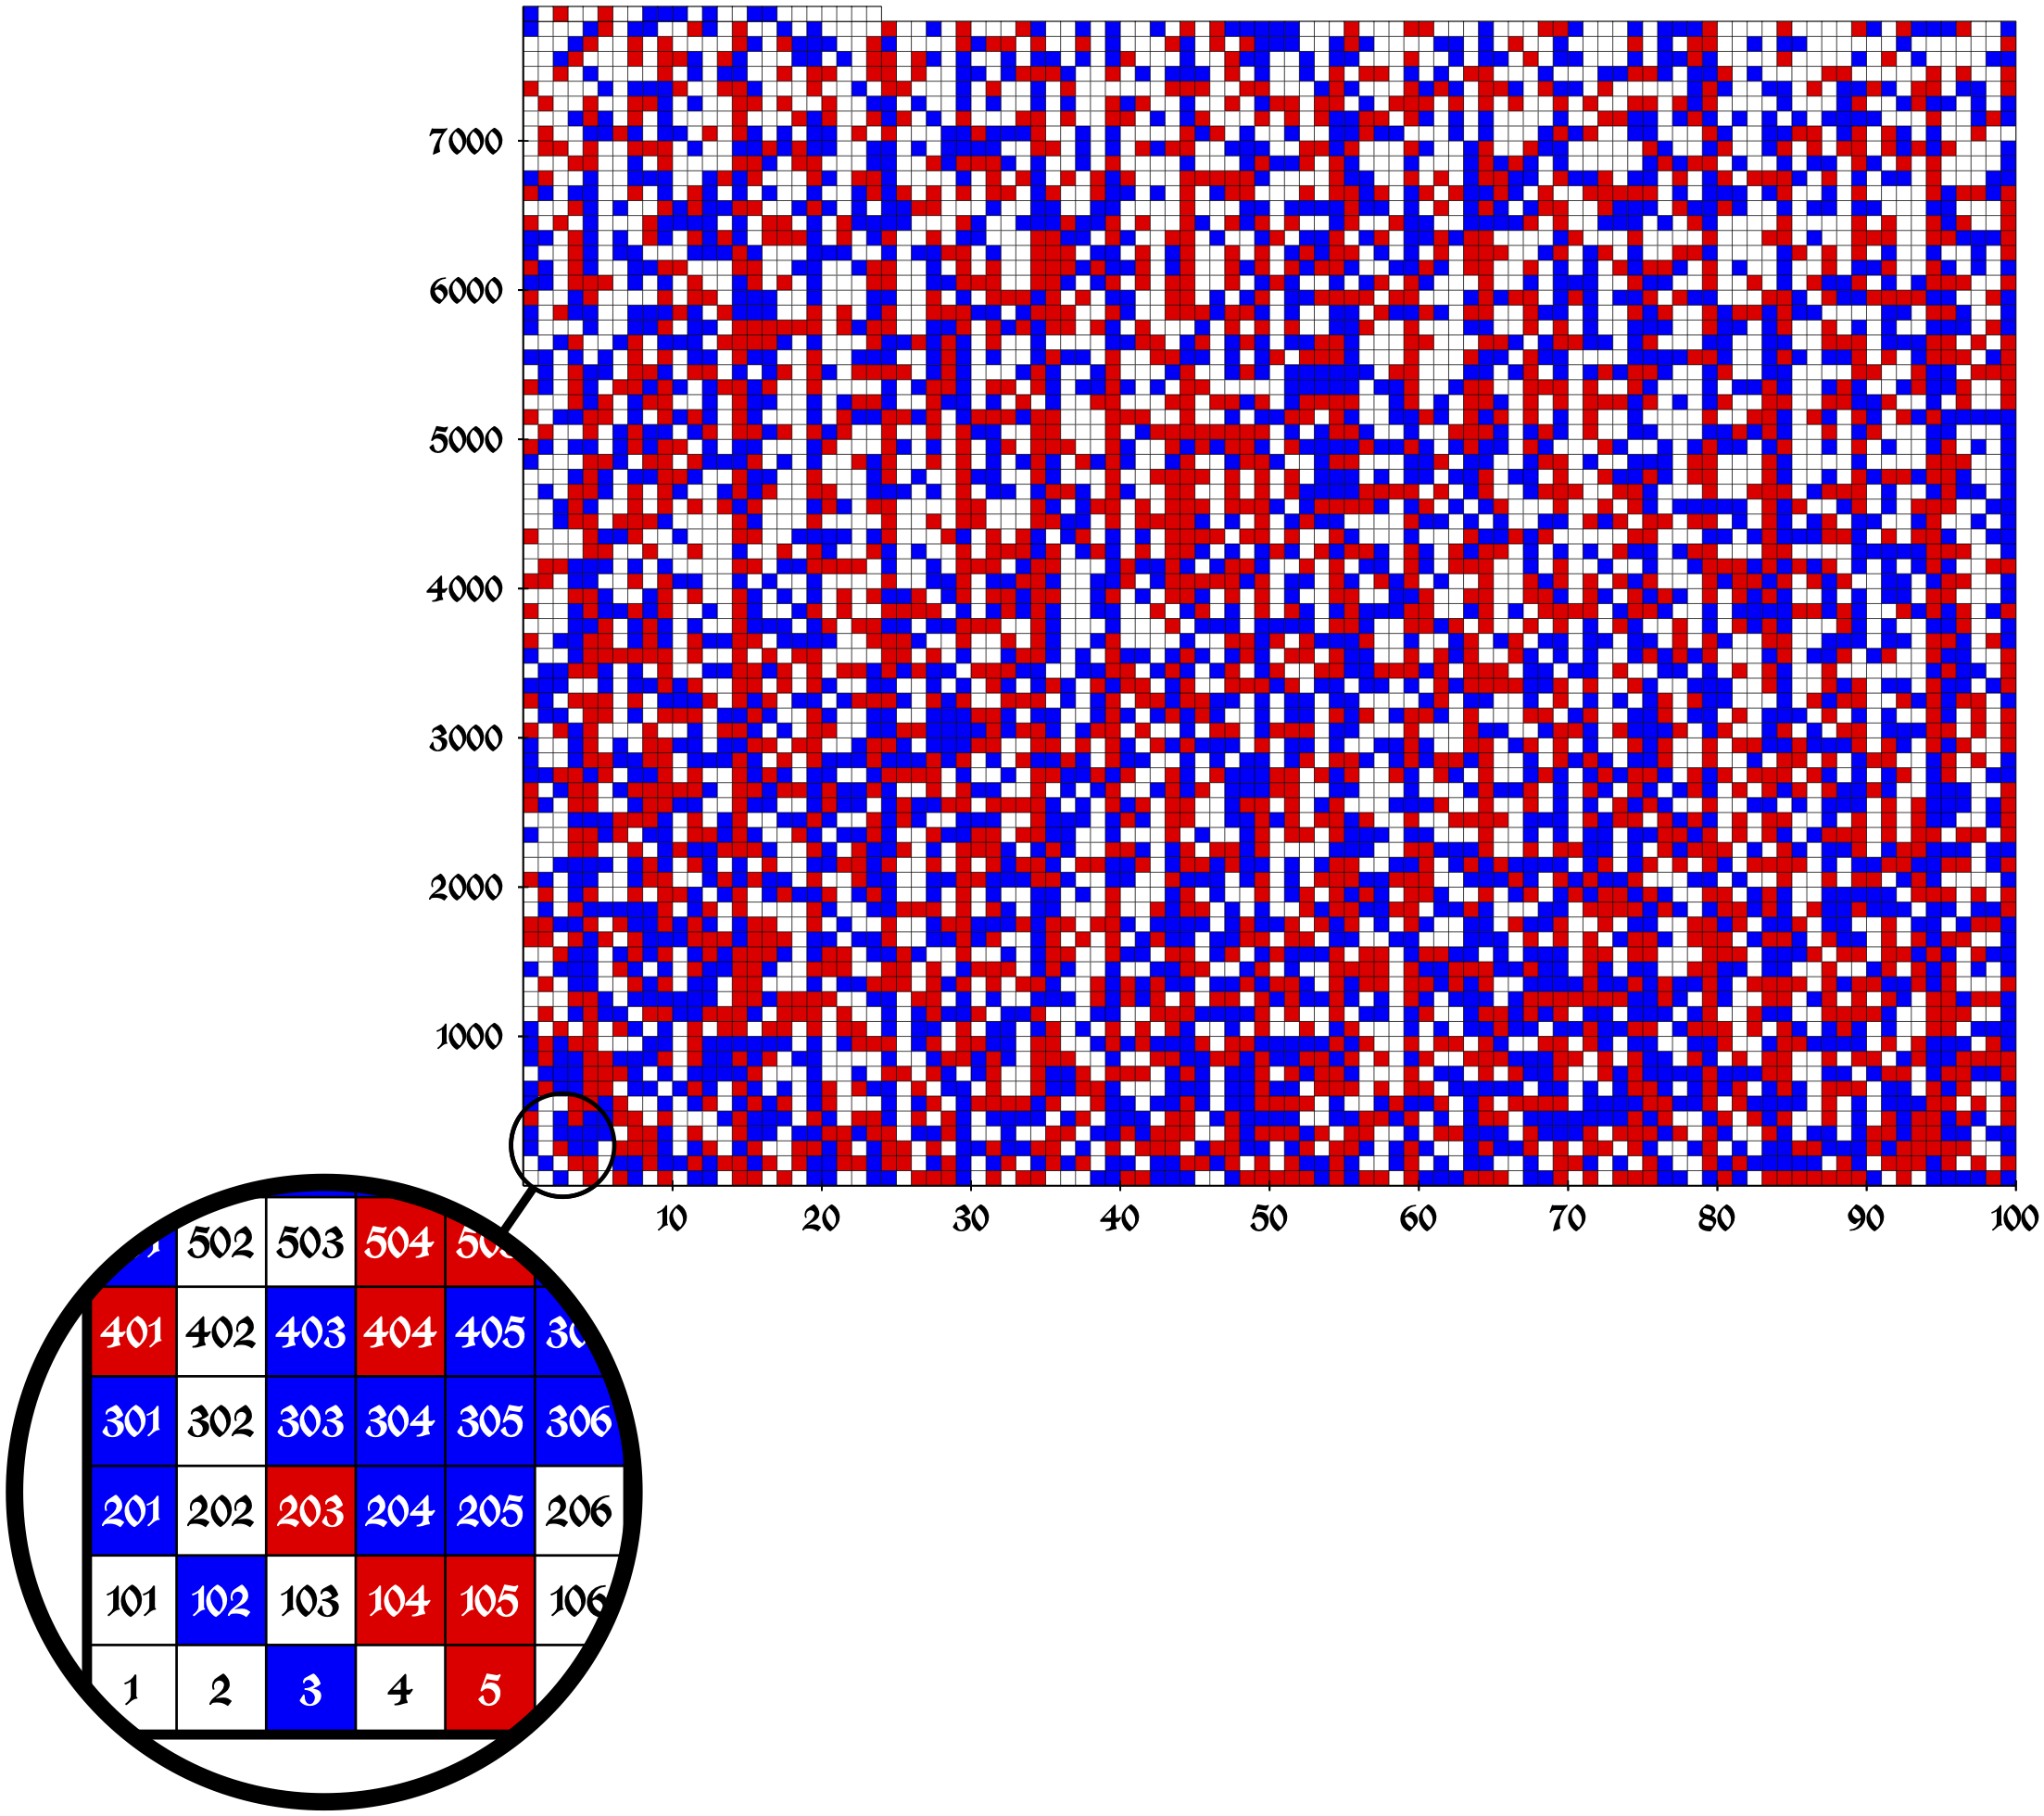
\includegraphics[scale=.27]{figs/PitagoreanTriples.png}
\end{column}
\begin{column}{0.5\textwidth}
Can all positive naturals be colored {\color{red}red} and
{\color{blue}blue}, so that all {\it Pythagorean
Triples} use  different colors?

A Pythagorean triple $(i, j, k)$ satisfies $i^2+j^2 = k^2$, as
$(3,4,5)$, and $(6,8,10)$.

Marijn Heule, Oliver Kullmann and Victor W. Marek \href{https://doi.org/10.1007/978-3-319-40970-2_15}{\color{blue}(SAT 2016)} solved the so called
{\bf Boolean Pythagorean triples problem} proving that such a
coloring is only possible up to the number $7824$. 
  
  \end{column}


\end{columns}

\end{frame}


\begin{frame}\frametitle{Formalizing Mathematics today}


  \begin{columns}
\begin{column}{0.35\textwidth}
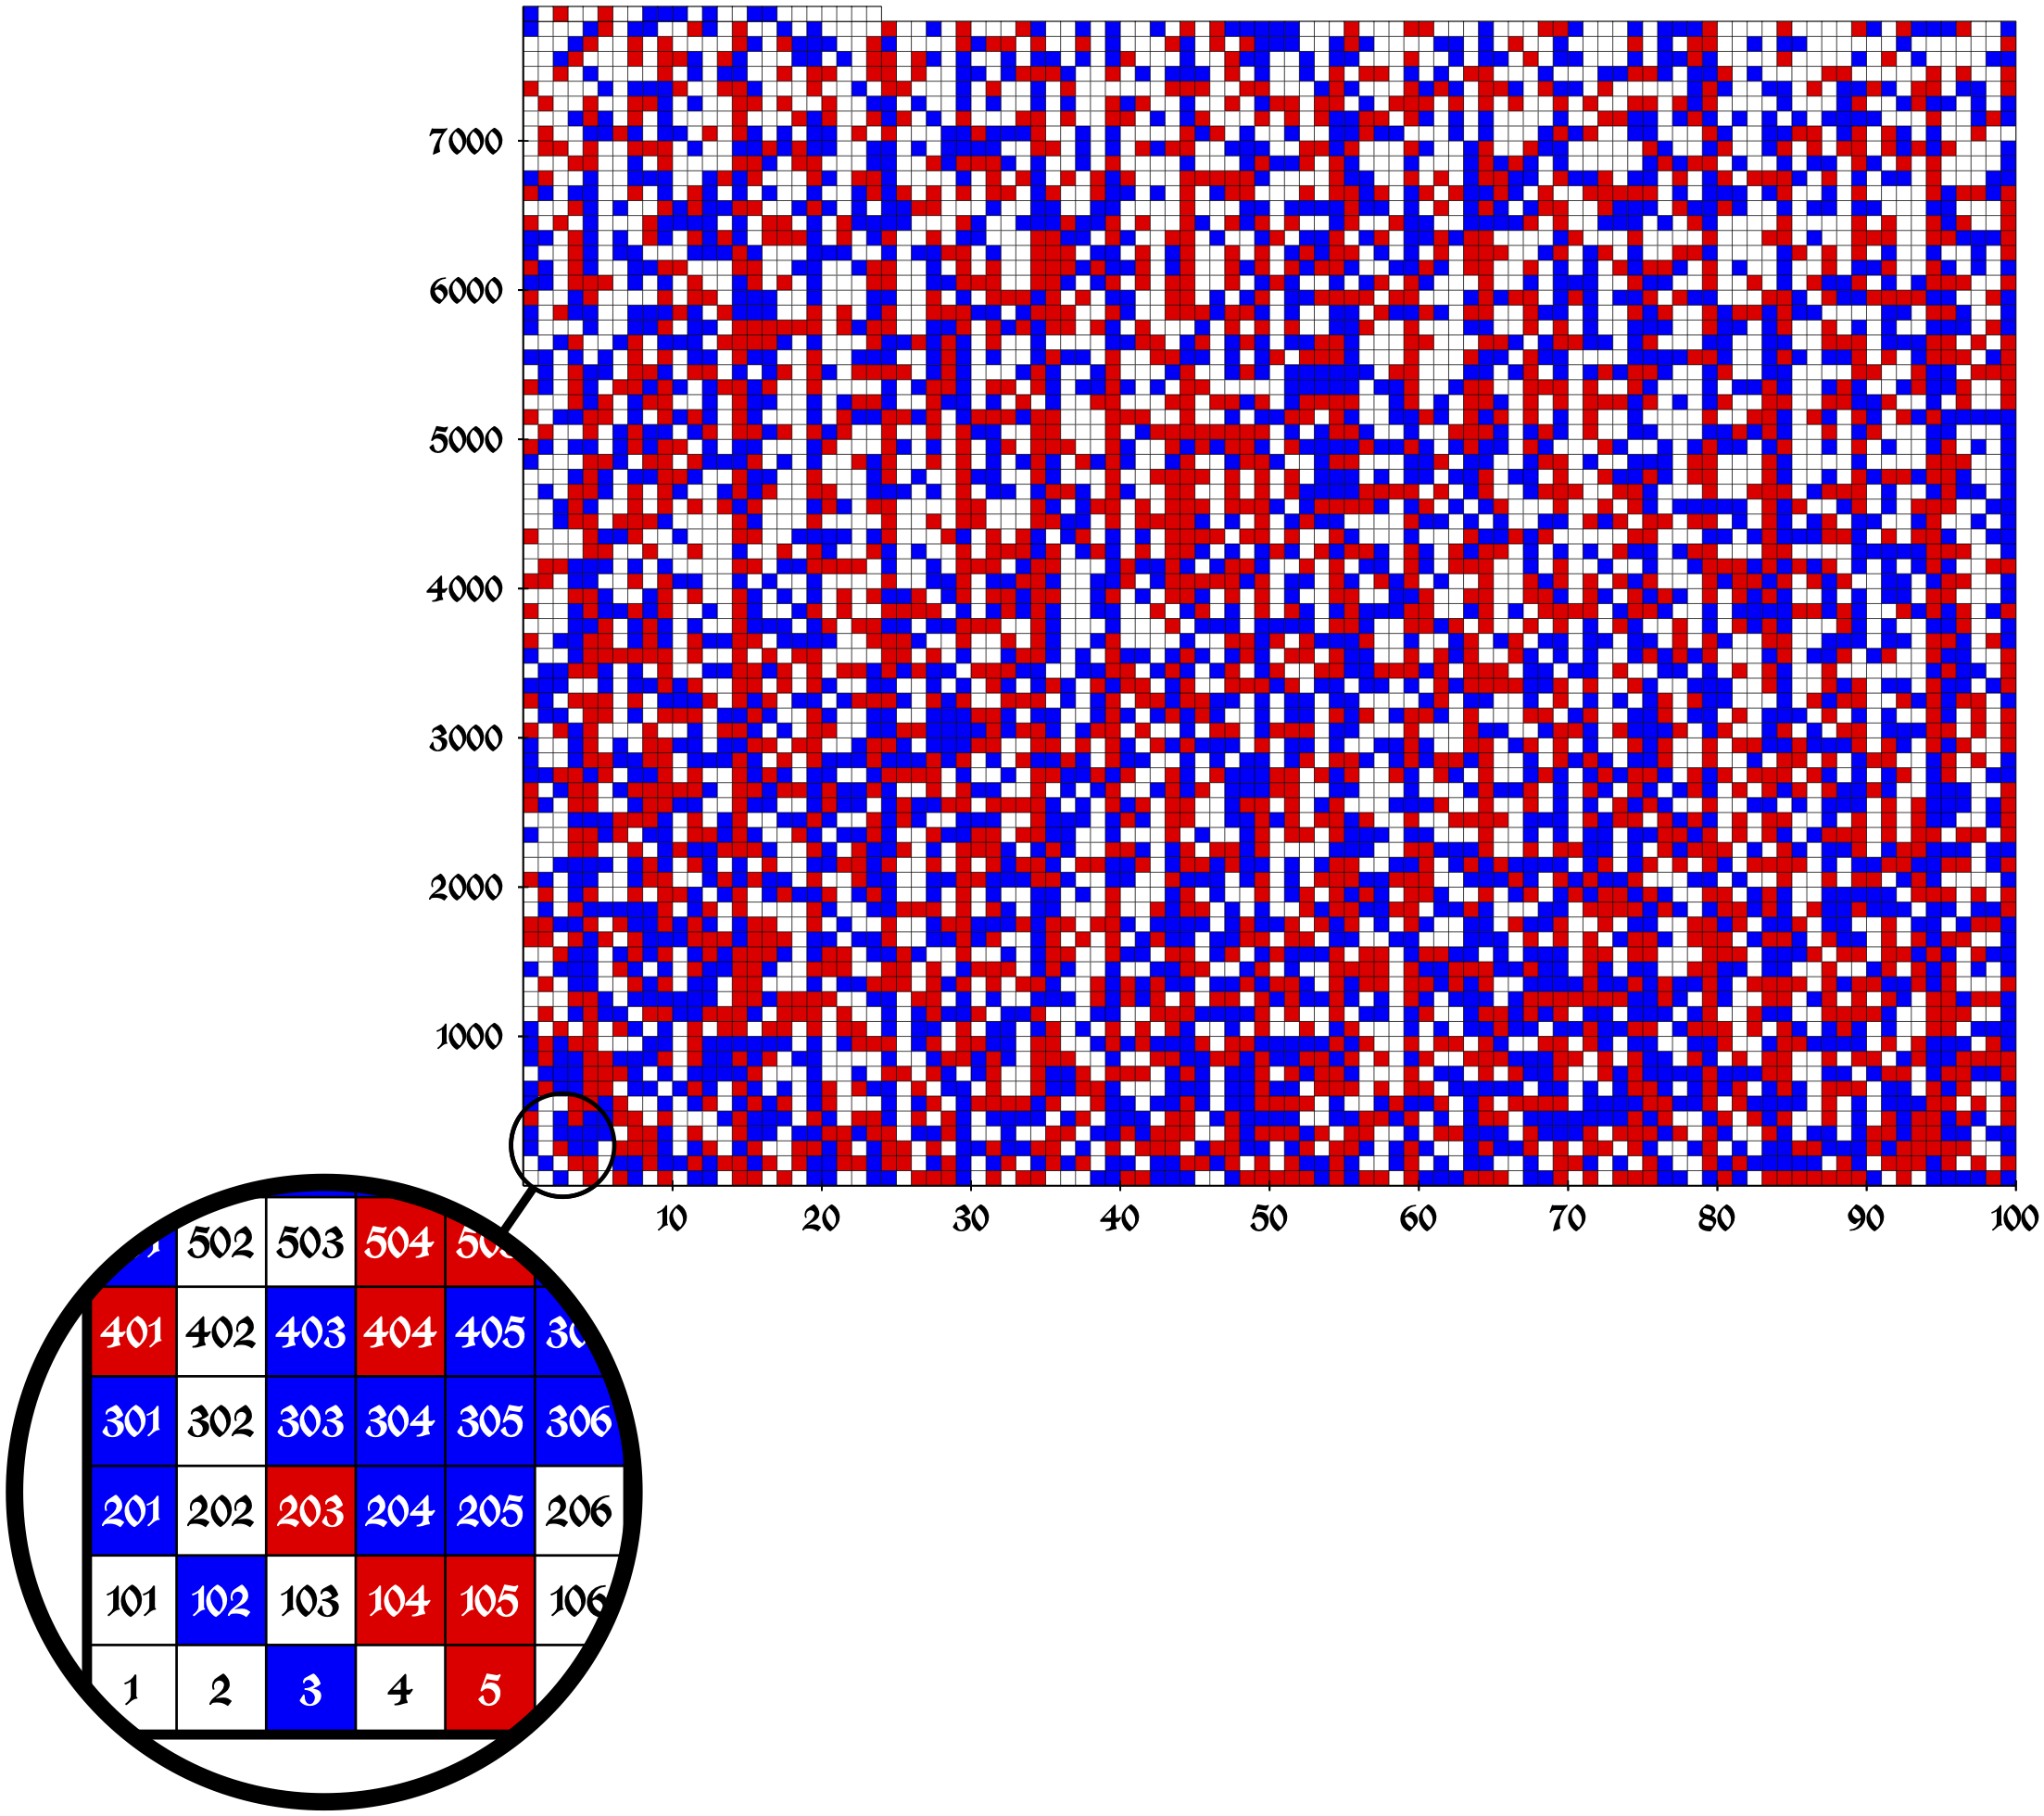
\includegraphics[scale=.24]{figs/PitagoreanTriples.png}
\end{column}
\begin{column}{0.6\textwidth}
 \small{ Essentially, they proved mechanically that $\Phi(n)$ holds for $n\leq
7824$, but not for $\Phi(7825)$, where:
\[\Phi(n) := \hspace{-5mm}\bigwedge_{\tiny\begin{array}{c}1\leq\! i\!<\!j\!<\!k\! \leq n\\ i^2+j^2 = k^2\end{array}}\hspace{-5mm} (x_i\vee
  x_j\vee x_k) \wedge  (\bar{x_i}\vee
  \bar{x_j}\vee \bar{x_k}) \]

Boolean solvers may be applied to prove satisfiability of
$\Phi(n)$ for $n\leq 7824$, but proving that unsatisfiability of
$\Phi(7825)$ required too much effort$^{\dag}$: checking that all of the
$2^{7825}$ possible bi-partitions of the set $\{1,\ldots,7825\}$
includes a Pythagorean triple in one of the two sets.   
}
  \end{column}
\end{columns}

\vspace{3mm}
\noindent$\mbox{}^\dag$\footnotesize{Creating the proof took
  about 4 CPU years on a cluster with 800 cores in about 2 days. It is
  \href{https://doi.org/10.1038/nature.2016.19990}{\color{blue}the largest proof ever}: almost 200 terabytes in size, from which it
  was extracted a compressed certificate of 68 gigabytes.}
\end{frame}




\begin{frame}\frametitle{Formalizing Mathematics}
Some related conferences/journals:

\vspace{1cm}

 \pgfuseimage{ITPcapa}  \hspace{5mm} \pgfuseimage{JARcapa}  \hspace{5mm} \pgfuseimage{TCScapa}  \hspace{5mm} \pgfuseimage{MSCScapa}  \hspace{5mm} 

\end{frame}


%==========================================================
%==========================================================
\begin{frame}[fragile]
\frametitle{Formalized Mathematics by GTC members}

\begin{itemize}
\item {\color{brown}Term Rewriting Theory}: 
  \href{https://github.com/nasa/pvslib/tree/master/TRS}{\color{blue}TRS}
  NASA PVS Library

\item {\color{brown}Program Termination}:
  \href{https://github.com/nasa/pvslib/tree/master/PVS0}{\color{blue}
    PVS0} and \href{https://github.com/nasa/pvslib/tree/master/CCG}{\color{blue} CCG}  NASA PVS Library

\item {\color{brown}Nominal Equational Reasoning}:
  \href{http://nominal.cic.unb.br}{\color{blue}Nominal} PVS theory

\item {\color{brown} Group and Ring's Theories}:
  \href{https://github.com/nasa/pvslib/tree/master/algebra}{\color{blue}Algebra}  NASA PVS Library

\end{itemize}

\end{frame}


%==========================================================
%==========================================================
\begin{frame}[fragile]
  \frametitle{Formalized Mathematics by GTC members: \\
   Term
      Rewriting theory -   \href{https://github.com/nasa/pvslib/tree/master/TRS}{\color{blue} TRS}
  \hfill  \href{http://trs.cic.unb.br}{\color{blue} trs.cic.unb.br}}

{\small
  \begin{itemize}

\item Termination | Ariane Alves
  Almeida (\href{https://repositorio.unb.br/handle/10482/42296}{\color{blue}PhD Informatics 2021})

\pgfuseimage{SciComProgCapita}  (2020) \href{https://doi.org/10.1016/j.scico.2020.102474}{\color{blue}\scriptsize\it ``Formalizing the Dependency Pair Criterion for Innermost Termination''}    
\item Confluence |
Andr\'e Luiz Galdino (\href{https://repositorio.unb.br/handle/10482/1343}{\color{blue}PhD Mathematics  2008}), Ana Cristina Oliveira (\href{https://repositorio.unb.br/handle/10482/22387}{\color{blue}PhD
Informatics  2016})

JFR (2008) \href{https://doi.org/10.6092/issn.1972-5787/1347}{\color{blue}\scriptsize\it   ``A Formalization of Newman's and
  Yokouchi's Lemmas in a Higher-Order Language''}

\pgfuseimage{JARcapita} (2017) \href{https://doi.org/10.1007/s10817-016-9376-2} {\color{blue}\scriptsize\it  ``Confluence of Orthogonal Term
Rewriting Systems in the Prototype Verification System''}


\item Knuth-Bendix Critical Pairs | 
Andr\'e Luiz Galdino (\href{https://repositorio.unb.br/handle/10482/1343}{\color{blue}PhD Mathematics  2008})

\pgfuseimage{JARcapita} (2010)  \href{https://doi.org/10.1007/s10817-010-9165-2}{\color{blue}\scriptsize\it ``A Formalization of the
Knuth-Bendix(-Huet) Critical Pair Theorem''}

\item Existence of First-order Unification |
Andr\'eia Borges Avelar (\href{https://repositorio.unb.br/handle/10482/18069}{\color{blue}PhD Math  2014})

\pgfuseimage{LJIGPLcapita} (2014)  \href{https://doi.org/10.1093/jigpal/jzu012}{\color{blue}\scriptsize\it ``First-order unification in the PVS proof assistant''} 


\end{itemize}
}
\end{frame}


%==========================================================
%==========================================================
\begin{frame}[fragile]
  \frametitle{Formalized Mathematics by GTC members:\\
   Program Termination Analysis -
   \href{https://github.com/nasa/pvslib/tree/master/PVS0}{\color{blue} PVS0} and  \href{https://github.com/nasa/pvslib/tree/master/CCG}{\color{blue} CCG}}

{\small
\begin{itemize}

\item Formalization of the Computational Theory of a functional
  language - \\ Thiago Ramos (PhD Informatics Student),
  Ariane Alves
  Almeida (\href{https://repositorio.unb.br/handle/10482/42296}{\color{blue}PhD Informatics 2021}), Andr\'eia Borges Avelar (\href{https://repositorio.unb.br/handle/10482/18069}{\color{blue}PhD Math  2014})
  Mariano Moscato \& C\'esar Mu\~noz, Aaron Dutle, Anthony Narkawicz  (NIA / NASA LaRC FM)

\pgfuseimage{WoLLICcapita} (2018)  \href{https://doi.org/10.1007/978-3-662-57669-4}{\color{blue}\scriptsize\it ``Formalization of the Undecidability of the Halting Problem for a Functional Language''}


\pgfuseimage{SciComProgCapita}  (2020) \href{https://doi.org/10.1016/j.scico.2020.102474}{\color{blue}\scriptsize\it ``Formalizing the Dependency Pair Criterion for Innermost Termination''}   

\pgfuseimage{JARcapita} (Submitted 2021)  \href{https://doi.org/10.4230/LIPIcs.ITP.2021.27}{\color{blue}\scriptsize\it
    ``Formal Verification of Termination Criteria for First-Order
    Recursive Functions''}. Presented in \pgfuseimage{LIPIcscapita}
  ITP  (2021) . 

\pgfuseimage{JARcapita}  (In press 2022) \href{https://doi.org/10.1007/s10817-021-09615-x}{\color{blue}\scriptsize\it
    ``Formalization of the Computational Theory of a Turing Complete Functional Language Model''} 

\end{itemize}
}  

\end{frame}







%==========================================================
%==========================================================
\begin{frame}[fragile]
  \frametitle{Formalized Mathematics by GTC members:\\
    Nominal Equational Reasoning \hfill \href{http://nominal.cic.unb.br}{\color{blue} nominal.cic.unb.br}}

{\color{blue} equality check}:    $s = t$? \hspace{.4cm}   {\color{blue} matching}: $\exists \sigma
  : s\sigma = t$? \hspace{.4cm}  {\color{blue} unification}: $\exists \sigma
  : s\sigma = t\sigma$?

{\footnotesize
\begin{itemize}

\item Formalization of Functional Nominal  Equality Check, matching, and Unification
  modulo C, A, and AC |  \\  Ana Cristina Oliveira (\href{https://repositorio.unb.br/handle/10482/22387}{\color{blue}PhD
Informatics  2016}), Washington de Carvalho Segundo
(\href{https://repositorio.unb.br/handle/10482/35474}{\color{blue}PhD Informatics
  2019}), Gabriel Silva (PhD Informatics student).

\pgfuseimage{ENTCScapita}  (2015)  \href{https://doi.org/10.1016/j.entcs.2016.06.005}{\color{blue}\scriptsize\it ``Completeness in PVS of a Nominal Unification Algorithm''}



\pgfuseimage{LOPSTRcapita} (2017)  \href{https://doi.org/10.1007/978-3-319-94460-9_14}{\color{blue}\scriptsize\it ``Nominal
  C-Unification''} 

\pgfuseimage{TCScapita} (2019) \href{https://doi.org/10.1016/j.tcs.2019.02.020}{\color{blue}\scriptsize\it ``A formalisation of nominal $\alpha$-equivalence with A, C, and AC function symbols''}

\pgfuseimage{LOPSTRcapita} (2019) \href{https://doi.org/10.1007/978-3-030-45260-5_8}{\color{blue}\scriptsize\it ``A Certified Functional Nominal C-Unification Algorithm''}

\pgfuseimage{MSCScapita}  (2021) \href{https://doi.org/10.1017/S0960129521000050}{\color{blue}\scriptsize\it ``Formalising nominal C-unification generalised with protected variables''}



\end{itemize}
}

\end{frame}



\begin{frame}[fragile]
  \frametitle{Formalized Mathematics by GTC members:\\
   Groups and Rings  \hfill \href{https://github.com/nasa/pvslib/tree/master/algebra}{\color{blue} algebra}}



{\footnotesize 
  \begin{itemize}
    
  \item  Thaynara A. de Lima (UFG), André Galdino (UFCat), Andréia
    Avelar (UnB), Mauricio Ayala-Rincón (UnB)


    \pgfuseimage{ITPcapita} (2018)
    \href{https://doi.org/10.1007/978-3-319-94821-8_3}{\color{blue}\scriptsize\it
      ``Formalizing Ring Theory in PVS ''}
    
    \pgfuseimage{JARcapita} (2021)
    \href{https://doi.org/10.1007/s10817-021-09593-0}{\color{blue}\scriptsize\it
        ``Formalization of Ring Theory in PVS - Isomorphism Theorems,
        Principal, Prime and Maximal Ideals,Chinese Remainder
        Theorem''}


\end{itemize}
}

\end{frame}


%==========================================================
%==========================================================
\begin{frame}[fragile]
\frametitle{Formalizing Mathematics at GTC (PPGs in Mathematics \& Informatics | UnB)}


You are welcome!

\vspace{1cm}

\pgfuseimage{LogforCScapa}\hspace{.3cm} \pgfuseimage{Logiccapa}
\hspace{.3cm} \pgfuseimage{Rewritingcapa}  \hspace{.3cm} \pgfuseimage{ProofTheorycapa}
\hspace{.3cm} \pgfuseimage{TypeTheorycapa} 



\end{frame}








\section{Gentzen's Calculus}



\begin{frame}
\frametitle{Gentzen Calculus}

\emph{Sequents}:

\[\begin{array}{ccc}
{\color{blue} \Gamma}&{\color{blue} \Rightarrow}&{\color{blue} \Delta}\\[5mm]
\uparrow && \uparrow\\
\mbox{antecedent}&&\mbox{succedent}\\
\end{array}\]
\end{frame}
%==========================================================
%==========================================================
\begin{frame}
\frametitle{Gentzen Calculus}

{\footnotesize
\begin{table}
\caption{\textsc{Rules of deduction \emph{\`a la} Gentzen for predicate logic}}
\label{rulesGentzenpredicatelogic}
\[\begin{array}{|c@{\hspace{1cm}}c|}
\hline
\mbox{{\color{red}Left rules}} & \mbox{{\color{red}Right rules}} \\
\hline 
\mbox{{\color{blue}Axioms:}}&\\[5mm]
\Gamma, \varphi \Rightarrow \varphi, \Delta\;\;(Ax)& 
\bot, \Gamma\Rightarrow\Delta\;\;(L_\bot)\\[5mm]
\hline
\mbox{{\color{blue}Structural rules:}}&\\[5mm]
\infer[(LW\mbox{\it eakening})]{\varphi,\Gamma\Rightarrow\Delta}{\Gamma\Rightarrow\Delta} & 
\infer[(RW\mbox{\it eakening})]{\Gamma\Rightarrow\Delta,\varphi}{\Gamma\Rightarrow\Delta}\\[5mm]
\infer[(LC\mbox{\it ontraction})]{\varphi,\Gamma\Rightarrow\Delta}{\varphi,\varphi,\Gamma\Rightarrow\Delta} & 
\infer[(RC\mbox{\it ontraction})]{\Gamma\Rightarrow\Delta,\varphi}{\Gamma\Rightarrow\Delta,\varphi,\varphi}\\[5mm]
\hline
\end{array}\]
\end{table}
}
\end{frame}
%==========================================================
%==========================================================
\begin{frame}
\frametitle{Gentzen Calculus}
{\tiny
\begin{table}
\caption{\textsc{Rules of deduction \emph{\`a la} Gentzen for predicate logic}}
\label{rulesGentzenpredicatelogicb}
\[\begin{array}{|c@{\hspace{1cm}}c|}
\hline
\mbox{{\color{red}Left rules}} & \mbox{{\color{red}Right rules}} \\
\hline
\mbox{{\color{blue}Logical rules:}}&\\[5mm]
\infer[(L_\wedge)]{\varphi_1\wedge\varphi_2,\Gamma\Rightarrow\Delta}{\varphi_{i\in\{1,2\}},\Gamma\Rightarrow\Delta} & 
\infer[(R_\wedge)]{\Gamma\Rightarrow\Delta,\varphi\wedge\psi}{\Gamma\Rightarrow\Delta,\varphi \;\; \Gamma\Rightarrow\Delta,\psi}\\[5mm]
\infer[(L_\vee)]{\varphi\vee\psi,\Gamma\Rightarrow\Delta}{\varphi,\Gamma\Rightarrow\Delta\;\;\psi,\Gamma\Rightarrow\Delta} & 
\infer[(R_\vee)]{\Gamma\Rightarrow\Delta,\varphi_1\vee\varphi_2}{\Gamma\Rightarrow\Delta, \varphi_{i\in\{1,2\}} }\\[5mm]
\infer[(L_\rightarrow)]{\varphi\rightarrow\psi,\Gamma\Rightarrow\Delta}{\Gamma\Rightarrow\Delta,\varphi\;\;\psi,\Gamma\Rightarrow\Delta} & 
\infer[(R_\rightarrow)]{\Gamma\Rightarrow\Delta,\varphi\rightarrow\psi}{\varphi,\Gamma\Rightarrow\Delta, \psi}\\[5mm]
\infer[(L_\forall)]{\forall_x \varphi, \Gamma\Rightarrow\Delta}{\varphi[x/t],\Gamma\Rightarrow\Delta} & 
\infer[(R_\forall),\;\;\;y\not\in \fv{\Gamma,\Delta}]{\Gamma\Rightarrow\Delta,\forall_x \varphi}{\Gamma\Rightarrow\Delta, \varphi[x/y]}\\[5mm]
\infer[(L_\exists),\;\;\;y\not\in \fv{\Gamma,\Delta}]{\exists_x\varphi,\Gamma\Rightarrow\Delta}{\varphi[x/y],\Gamma\Rightarrow\Delta} & 
\infer[(R_\exists)]{\Gamma\Rightarrow\Delta,\exists_x\varphi}{\Gamma\Rightarrow\Delta,\varphi[x/t]}\\[5mm]
\hline
\end{array}\]
\end{table}
}
\end{frame}
%==========================================================
%==========================================================
\begin{frame}
\frametitle{Gentzen Calculus}

Derivation of the Peirce's law:
${\color{red} \vdash ((\varphi \rightarrow \psi) \rightarrow \psi)
  \rightarrow \psi}$

 \begin{mathpar}
  %\inferrule*[Right={($L_\rightarrow$)}]
 % {\inferrule*[Right={($R_\rightarrow$)}]
 % {\inferrule*[Left={($R_\rightarrow$)}]{
\varphi\Rightarrow\varphi\;\;(Ax)
 % {\Rightarrow \varphi, \varphi\to\psi}}
    % \and \varphi\Rightarrow\varphi\;\;(Ax)}
  %{(\varphi\to\psi)\to\varphi\Rightarrow \varphi}}
  %{\Rightarrow ((\varphi\to\psi)\to\varphi)\to\varphi}
\end{mathpar}
\end{frame}
%==========================================================
%==========================================================
\begin{frame}
\frametitle{Gentzen Calculus}

Derivation of the Peirce's law:
${\color{red} \vdash ((\varphi \rightarrow \psi) \rightarrow \psi)
  \rightarrow \psi}$

 \begin{mathpar}
  %\inferrule*[Right={($L_\rightarrow$)}]
 % {\inferrule*[Right={($R_\rightarrow$)}]
 % {\inferrule*[Left={($R_\rightarrow$)}]{
  {\inferrule*[Left={($RW$)}]{\varphi\Rightarrow\varphi\;\;(Ax)}{\varphi\Rightarrow\varphi,\psi}}
 % {\Rightarrow \varphi, \varphi\to\psi}}
    % \and \varphi\Rightarrow\varphi\;\;(Ax)}
  %{(\varphi\to\psi)\to\varphi\Rightarrow \varphi}}
  %{\Rightarrow ((\varphi\to\psi)\to\varphi)\to\varphi}
\end{mathpar}
\end{frame}
%==========================================================
%==========================================================
\begin{frame}
\frametitle{Gentzen Calculus}

Derivation of the Peirce's law:
${\color{red} \vdash ((\varphi \rightarrow \psi) \rightarrow \psi)
  \rightarrow \psi}$

 \begin{mathpar}
  %\inferrule*[Right={($L_\rightarrow$)}]
 % {\inferrule*[Right={($R_\rightarrow$)}]
  {\inferrule*[Left={($R_\rightarrow$)}]{
  \inferrule*[Left={($RW$)}]{\varphi\Rightarrow\varphi\;\;(Ax)}{\varphi\Rightarrow\varphi,\psi}}
  {\Rightarrow \varphi, \varphi\to\psi}}
    % \and \varphi\Rightarrow\varphi\;\;(Ax)}
  %{(\varphi\to\psi)\to\varphi\Rightarrow \varphi}}
  %{\Rightarrow ((\varphi\to\psi)\to\varphi)\to\varphi}
\end{mathpar}
\end{frame}
%==========================================================
%==========================================================
\begin{frame}
\frametitle{Gentzen Calculus}

Derivation of the Peirce's law:
${\color{red} \vdash ((\varphi \rightarrow \psi) \rightarrow \psi)
  \rightarrow \psi}$

 \begin{mathpar}
  %\inferrule*[Right={($L_\rightarrow$)}]
 % {\inferrule*[Right={($R_\rightarrow$)}]
  {\inferrule*[Left={($R_\rightarrow$)}]{
  \inferrule*[Left={($RW$)}]{\varphi\Rightarrow\varphi\;\;(Ax)}{\varphi\Rightarrow\varphi,\psi}}
  {\Rightarrow \varphi, \varphi\to\psi}
     \and \varphi\Rightarrow\varphi\;\;(Ax)}
  %{(\varphi\to\psi)\to\varphi\Rightarrow \varphi}}
  %{\Rightarrow ((\varphi\to\psi)\to\varphi)\to\varphi}
\end{mathpar}
\end{frame}
%==========================================================
%==========================================================
\begin{frame}
\frametitle{Gentzen Calculus}

Derivation of the Peirce's law:
${\color{red} \vdash ((\varphi \rightarrow \psi) \rightarrow \psi)
  \rightarrow \psi}$

 \begin{mathpar}
  %\inferrule*[Right={($L_\rightarrow$)}]
  {\inferrule*[Right={($L_\rightarrow$)}]
  {\inferrule*[Left={($R_\rightarrow$)}]{
  \inferrule*[Left={($RW$)}]{\varphi\Rightarrow\varphi\;\;(Ax)}{\varphi\Rightarrow\varphi,\psi}}
  {\Rightarrow \varphi, \varphi\to\psi}
     \and \varphi\Rightarrow\varphi\;\;(Ax)}
  {(\varphi\to\psi)\to\varphi\Rightarrow \varphi}}
  %{\Rightarrow ((\varphi\to\psi)\to\varphi)\to\varphi}
\end{mathpar}
\end{frame}

%==========================================================
%==========================================================
\begin{frame}
\frametitle{Gentzen Calculus}

Derivation of the Peirce's law:
${\color{red} \vdash ((\varphi \rightarrow \psi) \rightarrow \psi)
  \rightarrow \psi}$

 \begin{mathpar}
  \inferrule*[Right={($L_\rightarrow$)}]
  {\inferrule*[Right={($L_\rightarrow$)}]
  {\inferrule*[Left={($R_\rightarrow$)}]
{\inferrule*[Left={($RW$)}]{\varphi\Rightarrow\varphi\;\;(Ax)}{\varphi\Rightarrow\varphi,\psi}}
  {\Rightarrow \varphi, \varphi\to\psi}
     \and \varphi\Rightarrow\varphi\;\;(Ax)}
  {(\varphi\to\psi)\to\varphi\Rightarrow \varphi}}
  {\Rightarrow ((\varphi\to\psi)\to\varphi)\to\varphi}
\end{mathpar}
\end{frame}
%==========================================================
%==========================================================
\begin{frame}
\frametitle{Gentzen Calculus}

Derivation of:
${\color{red} \vdash \exists_x \neg \varphi \Rightarrow \neg
  \forall_x\varphi}$

\begin{mathpar}
\inferrule*[Right={($L_\exists$)}]
{\inferrule*[Right={(c-equiv)}]
{\inferrule*[Right={(c-equiv)}]
{\inferrule*[Left={($L_{\forall}$)}]
{\varphi[x/t] \Rightarrow \varphi[x/t]} 
{\forall_x \varphi \Rightarrow \varphi[x/t]}}
{\neg \varphi[x/t], \forall_x\varphi \Rightarrow}}
{\neg \varphi[x/t] \Rightarrow \neg \forall_x \varphi}}
{\exists_x \neg \varphi \Rightarrow \neg \forall_x \varphi}
\end{mathpar}
\end{frame}
%==========================================================
%==========================================================

\begin{frame}
\frametitle{Gentzen Calculus}

\emph{{\color{blue}Cut rule}}:
 \[\begin{array}{|c|}
\hline
\\
\infer[(Cut)]{\Gamma\Gamma'\Rightarrow\Delta\Delta'}{\Gamma\Rightarrow\Delta,\varphi\;\;\;\varphi,\Gamma'\Rightarrow\Delta'}\\[5mm]
\hline
\end{array} 
\]

\end{frame}
%==========================================================
%==========================================================

\begin{frame}
\frametitle{Gentzen Calculus - dealing with negation: $c$-equivalence}

\[\varphi,\Gamma\Rightarrow\Delta \mbox{ one-step c-equivalent }
\Gamma\Rightarrow\Delta,\neg\varphi\]

\[\Gamma\Rightarrow\Delta, \varphi \mbox{ one-step c-equivalent }
\neg\varphi,\Gamma\Rightarrow\Delta\]

The {\color{blue}c-equivalence}  is the equivalence closure of this relation.

\begin{lemma}[One-step c-equivalence]
\begin{enumerate}[(i)]
\item $\vdash_G\varphi, \Gamma\Rightarrow\Delta$, iff 
$\vdash_G\Gamma\Rightarrow\Delta, \neg\varphi$;
\item $\vdash_G\neg\varphi, \Gamma\Rightarrow\Delta$, iff
 $\vdash_G\Gamma\Rightarrow\Delta, \varphi$.
\end{enumerate}
\end{lemma}
\end{frame}

%==========================================================
%==========================================================

\begin{frame}
\frametitle{Gentzen Calculus - dealing with negation}
\footnotesize{

\hspace{-1mm}\begin{minipage}{0.9\textwidth}
\noindent{\it \color{blue}Proof.} 
\begin{enumerate}[(i)]
\item {\bf Necessity}:
 \begin{mathpar}
\inferrule*[Right={(R$_\to$)}]{
\inferrule*[Right={(RW)}]{
\varphi,\Gamma\Rightarrow\Delta
}
{\varphi,\Gamma\Rightarrow\Delta,\bot}}
{\Gamma\Rightarrow\Delta,\neg\varphi}
\end{mathpar}

{\bf Sufficiency}: 
\begin{mathpar}
\inferrule*[Right={(Cut)}]{
\inferrule*[Left={(LW)}]{
\Gamma\Rightarrow\Delta,\neg\varphi
}
{\varphi,\Gamma\Rightarrow\Delta,\neg\varphi}
\and \and
\inferrule*[Right={(L$_\to$)}]{
(Ax) \;\varphi,\Gamma\Rightarrow\Delta,\varphi \and 
\bot, \varphi,\Gamma\Rightarrow\Delta  \; (L_\bot)
}
{\neg\varphi,\varphi,\Gamma\Rightarrow\Delta}
}
{\varphi,\Gamma\Rightarrow\Delta}
\end{mathpar}

\end{enumerate}
\end{minipage}
}
\end{frame}
%==========================================================
%==========================================================

\begin{frame}
\frametitle{Gentzen Calculus - dealing with negation}

\hspace{-4mm}\begin{minipage}{0.95\textwidth}
\footnotesize{ 
\begin{enumerate}[(ii)]
\item {\bf Necessity}:

{\tiny
\begin{mathpar}
\inferrule*[Right={{\tiny  (Cut)}}]{
\inferrule*[Left={{\tiny (R$_\to$)}}]{
\inferrule*[Left={{\tiny  (L$_\to$)}}]{
\inferrule*[Left={{\tiny  (R$_\to$)}}]{
(Ax)\;\varphi,\Gamma\Rightarrow\Delta,\varphi,\varphi,\bot}
{\Gamma\Rightarrow\Delta,\varphi,\varphi,\neg\varphi}
\;
\bot, \Gamma\Rightarrow\Delta, \varphi,\varphi  \; (L_\bot)}
{\neg\neg\varphi,\Gamma\Rightarrow\Delta,\varphi,\varphi}}
{\Gamma\Rightarrow\Delta, \varphi, \neg\neg\varphi\to\varphi}
\;\; 
\inferrule*[Right={{\tiny  (L$_\to$)}}]{
\inferrule*[Right={{\tiny  (R$_\to$)}}]{
\inferrule*[Right={{\tiny  (RW)}}]{
\neg\varphi,\Gamma\Rightarrow\Delta}
{\neg\varphi,\Gamma\Rightarrow\Delta,\varphi,\bot}}
{\Gamma\Rightarrow\Delta,\varphi,\neg\neg\varphi}
\and \\
\varphi,\Gamma\Rightarrow\Delta,\varphi\; (Ax)
}
{\neg\neg\varphi\to\varphi,\Gamma\Rightarrow\Delta,\varphi}
}
{\Gamma\Rightarrow\Delta,\varphi}
\end{mathpar}
}

{\bf Sufficiency}: 

\begin{mathpar}
\inferrule*[Right={(L$_\to$)}]{
\Gamma\Rightarrow \Delta,\varphi
\and
\bot,\Gamma \Rightarrow \Delta}
{\neg\varphi,\Gamma\Rightarrow\Delta}
\end{mathpar}

\end{enumerate}

\mbox{}\hfill{\color{blue}$\Box$}
}
\end{minipage}
\end{frame}


\end{document}
%==========================================================
%==========================================================
%==========================================================
